\begin{frame}		
	\frametitle{Sliding Window}
	\framesubtitle{Selective Repeat. Principle}
	
	\begin{figure}[H]
		\center{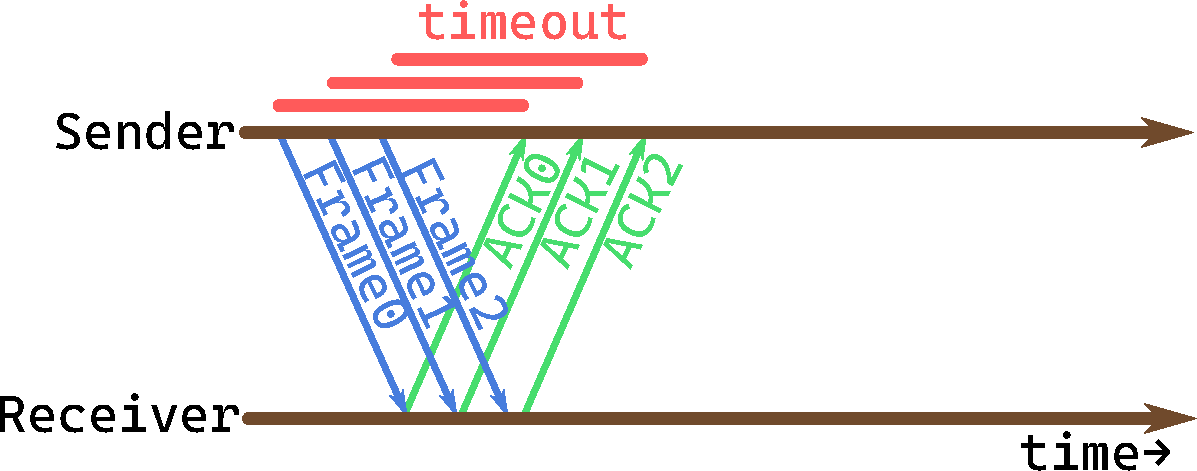
\includegraphics[width = 1\textwidth]{sr-1}}
	\end{figure}
	
	\footnotetext{Demo: \href{https://www2.tkn.tu-berlin.de/teaching/rn/animations/}{1}, \href{https://wps.pearsoned.com/ecs_kurose_compnetw_6/216/55463/14198702.cw/index.html}{2}}
\end{frame}

\begin{frame}		
	\frametitle{Sliding Window}
	\framesubtitle{Selective Repeat. Principle}
	
	\begin{figure}[H]
		\center{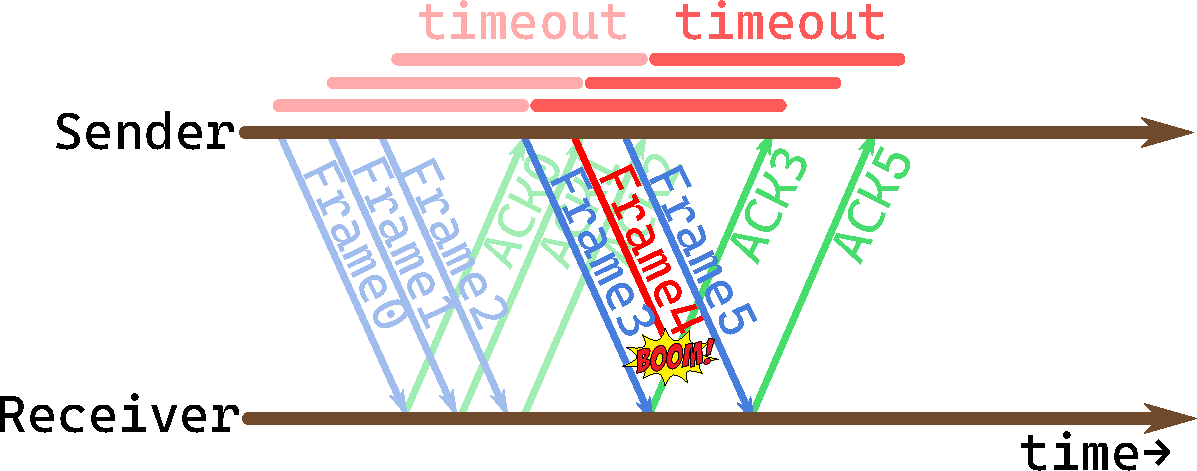
\includegraphics[width = 1\textwidth]{sr-2}}
	\end{figure}
	
	\footnotetext{Demo: \href{https://www2.tkn.tu-berlin.de/teaching/rn/animations/}{1}, \href{https://wps.pearsoned.com/ecs_kurose_compnetw_6/216/55463/14198702.cw/index.html}{2}}
\end{frame}

\begin{frame}		
	\frametitle{Sliding Window}
	\framesubtitle{Selective Repeat. Principle}
	
	\begin{figure}[H]
		\center{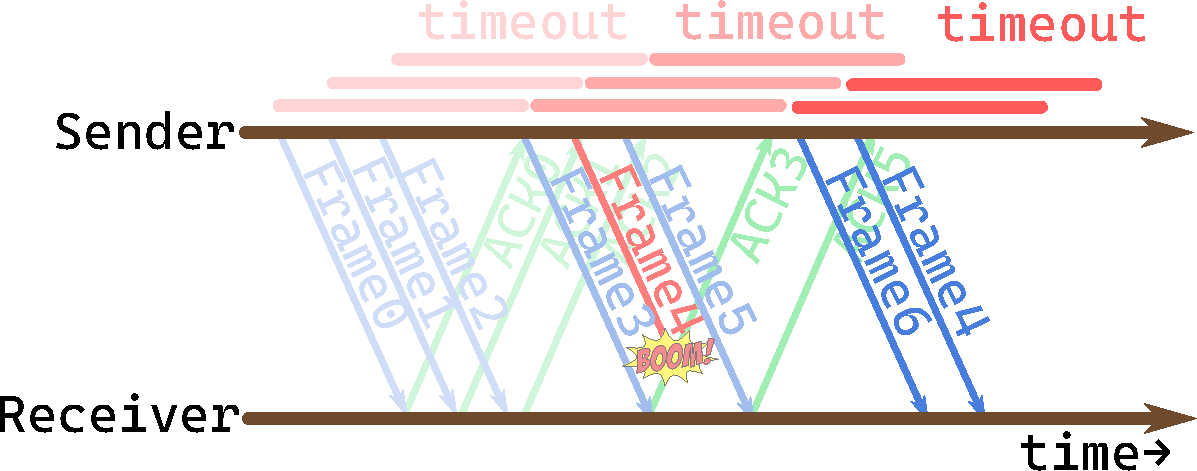
\includegraphics[width = 1\textwidth]{sr-3}}
	\end{figure}
	
	\footnotetext{Demo: \href{https://www2.tkn.tu-berlin.de/teaching/rn/animations/}{1}, \href{https://wps.pearsoned.com/ecs_kurose_compnetw_6/216/55463/14198702.cw/index.html}{2}}
\end{frame}


\begin{frame}		
	\frametitle{Sliding Window}
	\framesubtitle{Efficiency of Selective Repeat}
	
	\begin{itemize}
		\item Probability of Failure: $P_f = plr$
		\item Average total time to transmit a packet [\cite{1}]. Windows size $W_s$ should be selected so that the channel will be busy all the time.
		$$E[t_{packet}] = \dfrac{ t_f }{1 - P_f}$$
		\item Effective information transmission rate: $R_{eff} =\dfrac{n_f - n_{headers}}{E[t_{packet}]} $
		\item Associated transmission efficiency: $\eta = \dfrac{R_{eff}}{Rate}$
\end{itemize}

\end{frame}


\begin{frame}		
	\frametitle{Sliding Window}
	\framesubtitle{Efficiency of Selective Repeat}
	
	\begin{columns}
		\begin{column}{0.5\textwidth}  %%<--- here
			\begin{center}
				\begin{figure}[H]
					\center{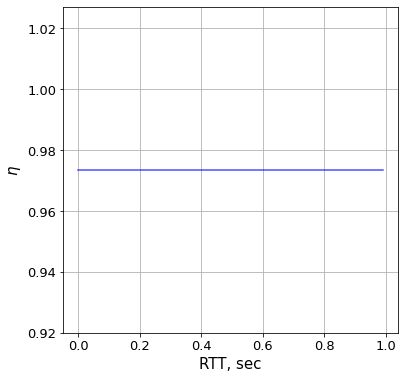
\includegraphics[width = 1\textwidth]{sr-rtt}}
				\end{figure}
			\end{center}
			\centering 
		\end{column}
		\begin{column}{0.5\textwidth}  %%<--- here
			\begin{center}
				\begin{figure}[H]
					\center{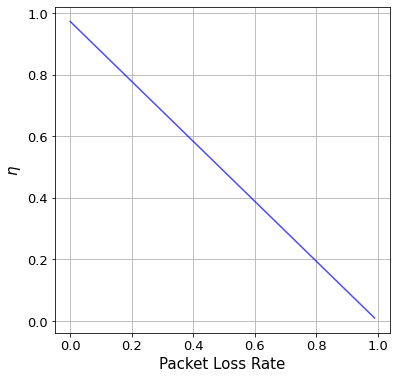
\includegraphics[width = 1\textwidth]{sr-plr}}
				\end{figure}
			\end{center}
			\centering 
		\end{column}
	\end{columns}
	
	
\end{frame}